\lecture{6}{13 Oct.}{}

\begin{recall}
    \(R^{(k)}(t)\) is the least \(n\) s.t.\ every red/blue coloring of \(\binom{[n]}{k}\) has a monochromatic \(t\)-set, and it grows like a tower of exponentials in \(t\). Equivalently, in a coloring of \(K_n^{(k)}\) the largest monochromatic set we can guarantee has size only \(O(\underbrace{\log \log \cdots \log}_{k-2 \text{ times}} n)\); see \autoref{sec:ramsey-counting}.
\end{recall}

\section{Finding a Dominant Color}\label{sec:dominant-color}

Demanding that \emph{all} \(\binom{t}{k}\) edges inside a \(t\)-set receive one color is a very strong requirement, and the previous section showed how badly it limits \(t\). This lecture proves that a much weaker requirement --- one color on a fixed proportion above a half --- is satisfied by sets that are larger by a tower of exponentials.

\begin{theorem}\label{thm:dominant-color}
    Suppose we two-color the edges of a complete \(k\)-uniform hypergraph on \(n\) vertices. Then there is a set \(S\) of \(\Omega\bigl( (\log n)^{1/(k-1)} \bigr)\) vertices s.t.\ a \(\bigl( \frac{1}{2} + c_k \bigr)\)-proportion of its edges receive the same color, for some constant \(c_k > 0\).
\end{theorem}

So the two conclusions live on completely different scales: insisting on all edges of \(S\) having one color forces \(S\) to be of iterated logarithmic size, while asking only for a fixed advantage over \(\frac{1}{2}\) allows \(S\) to be polylogarithmic in \(n\).
\begin{center}
    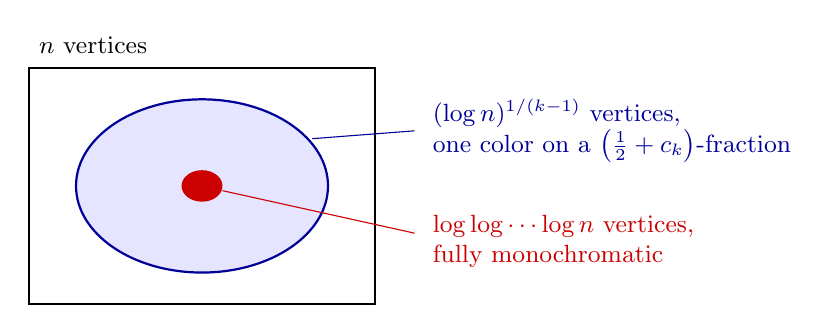
\begin{tikzpicture}[thick, every node/.style={font=\small}]
        \draw (0,0) rectangle (4.4,3.0);
        \node[anchor=south west] at (0,3.05) {$n$ vertices};
        \fill[blue!10] (2.2,1.5) ellipse (1.6 and 1.1);
        \draw[blue!60!black] (2.2,1.5) ellipse (1.6 and 1.1);
        \node[blue!60!black, anchor=west, align=left] at (5.0,2.2)
            {$(\log n)^{1/(k-1)}$ vertices,\\one color on a $\bigl( \frac{1}{2} + c_k \bigr)$-fraction};
        \fill[red!80!black] (2.2,1.5) ellipse (0.26 and 0.2);
        \node[red!80!black, anchor=west, align=left] at (5.0,0.8)
            {$\log \log \cdots \log n$ vertices,\\fully monochromatic};
        \draw[blue!60!black, thin] (3.6,2.1) -- (4.9,2.2);
        \draw[red!80!black, thin] (2.46,1.44) -- (4.9,0.9);
    \end{tikzpicture}
\end{center}

The proof has two ingredients: a structural theorem of Erd\H{o}s, which supplies a configuration on which one color is already guaranteed, and an analytic lemma about polynomials, which is what converts that configuration into a dominant color.

\subsection{Erd\H{o}s's Transversal Theorem}

\begin{theorem}[Erd\H{o}s]\label{thm:erdos-transversal}
    Given any red/blue coloring of \(E(K_n^{(k)})\), there exist \(k\) pairwise disjoint subsets \(A_1, \ldots, A_k\) of \([n]\), each of size
    \[
        m = \Omega\bigl( (\log n)^{1/(k-1)} \bigr),
    \]
    s.t.\ every edge \(e\) with \(\abs{e \cap A_i} = 1\) for all \(i\) receives the same color.
\end{theorem}

Call an edge meeting each \(A_i\) exactly once a \vocab{transversal} edge; there are \(m^k\) of them, one for each choice of a vertex from each part, and the theorem says they are monochromatic as a family.
\begin{center}
    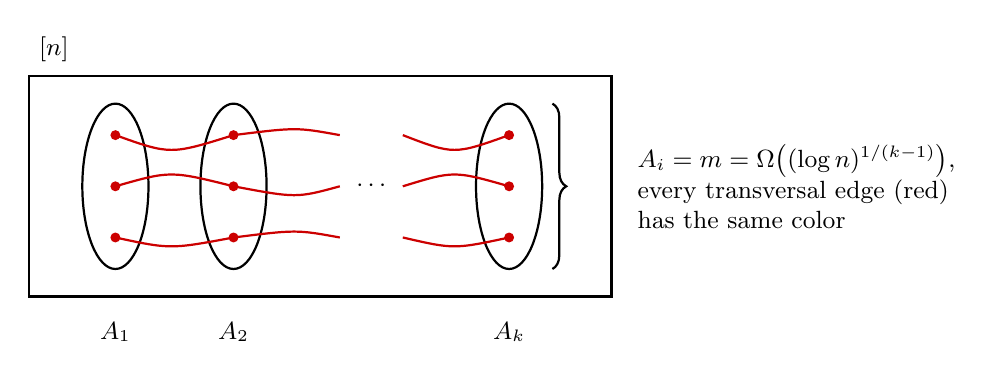
\begin{tikzpicture}[thick, every node/.style={font=\small}]
        \draw (0,-0.3) rectangle (7.4,2.5);
        \node[anchor=south west] at (0,2.55) {$[n]$};
        \foreach \x/\lab in {1.1/{A_1}, 2.6/{A_2}, 6.1/{A_k}} {
            \draw (\x,1.1) ellipse (0.42 and 1.05);
            \node at (\x,-0.75) {$\lab$};
        }
        \node at (4.35,1.1) {$\cdots$};
        \foreach \y/\yy/\yyy in {1.75/1.5/1.85, 1.1/1.3/0.95, 0.45/0.3/0.55} {
            \draw[red!80!black] (1.1,\y) .. controls (1.8,\yy) .. (2.6,\y)
                                (2.6,\y) .. controls (3.4,\yyy) .. (3.95,\y);
            \draw[red!80!black] (4.75,\y) .. controls (5.4,\yy) .. (6.1,\y);
            \fill[red!80!black] (1.1,\y) circle (1.8pt);
            \fill[red!80!black] (2.6,\y) circle (1.8pt);
            \fill[red!80!black] (6.1,\y) circle (1.8pt);
        }
        \draw[decorate, decoration={brace, amplitude=5pt}] (6.65,2.15) -- (6.65,0.05);
        \node[anchor=west, align=left] at (7.6,1.1)
            {$\abs{A_i} = m = \Omega\bigl( (\log n)^{1/(k-1)} \bigr)$,\\every transversal edge (red)\\has the same color};
    \end{tikzpicture}
\end{center}

\begin{remark}
    Nothing is claimed about the other edges, those meeting some \(A_i\) in \(0\) or in \(\ge 2\) vertices; they may be colored arbitrarily. This is exactly why \autoref{thm:erdos-transversal} can afford parts of size \((\log n)^{1/(k-1)}\), so much larger than the monochromatic sets of \autoref{sec:ramsey-counting}: a transversal family is a far weaker demand than a clique.
\end{remark}

\subsection{A Polynomial Lemma}

The second ingredient looks unrelated at first, and we state it before explaining where it is used.

\begin{lemma}\label{lem:polynomial}
    Let \(k \in \mathbb{N}\), and let \(\mathcal{P}_k\) be the set of homogeneous polynomials in \(x_1, x_2, \ldots, x_k\) of degree \(k\) whose coefficients lie in \([-1,1]\) and whose coefficient of \(x_1 x_2 \cdots x_k\) is \(1\). Then there is a constant \(c_k > 0\) s.t.
    \[
        \forall\, f \in \mathcal{P}_k \ \ \exists\, (x_1, \ldots, x_k) \in [0,1]^k \ \text{ s.t. } \ \abs{f(x_1, \ldots, x_k)} \ge c_k.
    \]
\end{lemma}

The content is the uniformity in \(f\): for each single \(f\) the existence of such a point is obvious, since \(f \not\equiv 0\); the lemma says one constant works for the whole family.

\begin{proof}
    Given \(f \in \mathcal{P}_k\), let
    \[
        M(f) = \max_{x_1, \ldots, x_k \in [0,1]} \abs{f(x_1, \ldots, x_k)},
    \]
    which exists because \(f\) is continuous and \([0,1]^k\) is compact. Since the coefficient of \(x_1 \cdots x_k\) is \(1\) we have \(f \not\equiv 0\), and a non-zero polynomial cannot vanish on all of \([0,1]^k\),\footnote{Write \(f = \sum_j g_j(x_1, \ldots, x_{k-1}) \, x_k^{\,j}\). By induction on \(k\) there are values of \(x_1, \ldots, x_{k-1}\) in \([0,1]\) at which some \(g_j\) is non-zero; fixing them turns \(f\) into a non-zero polynomial in \(x_k\) alone, which vanishes at only finitely many \(x_k\). The ``finitely many roots'' step is available for one variable only: in \(k \ge 2\) variables the zero set is a hypersurface, e.g.\ \(x_1 - x_2\) vanishes along a diagonal of \([0,1]^2\).} so \(M(f) > 0\).

    Next, \(\mathcal{P}_k\) is compact. Writing \(D = \binom{2k-1}{k}\) for the number of degree-\(k\) monomials in \(x_1, \ldots, x_k\), a member of \(\mathcal{P}_k\) is determined by its \(D-1\) free coefficients, the coefficient of \(x_1 \cdots x_k\) being fixed to \(1\). This gives a map
    \[
        \Phi \colon [-1,1]^{D-1} \longrightarrow C\bigl( [0,1]^k \bigr), \qquad \text{coefficients} \longmapsto \text{the polynomial they define},
    \]
    whose image is exactly \(\mathcal{P}_k\). It is continuous for the supremum norm, since every monomial is bounded by \(1\) on \([0,1]^k\) and hence \(\norm{\Phi(a) - \Phi(b)}_\infty \le D \max_i \abs{a_i - b_i}\). A continuous image of a compact set is compact, so \(\mathcal{P}_k\) is compact; and \(M = \norm{\cdot}_\infty\) is continuous.

    So \(M\) attains its minimum on \(\mathcal{P}_k\), i.e.\ there is \(f_0 \in \mathcal{P}_k\) with
    \[
        \min_{f \in \mathcal{P}_k} M(f) = M(f_0) \eqqcolon c_k > 0,
    \]
    and this \(c_k\) works for every \(f \in \mathcal{P}_k\).
\end{proof}

\subsection{Proof of the Theorem}

\begin{proof}[Proof of \autoref{thm:dominant-color}]
    By \autoref{thm:erdos-transversal} there are pairwise disjoint \(A_1, \ldots, A_k\) of size \(m = \Omega\bigl( (\log n)^{1/(k-1)} \bigr)\) s.t.\ every edge \(e\) with \(\abs{e \cap A_i} = 1\) for all \(i\) is, without loss of generality, colored blue.

    \textbf{The coloring as a \(\pm 1\) function.} Think of the coloring as a map \(\chi \colon E \to \{\pm 1\}\),
    \[
        \chi(e) =
        \begin{cases}
            +1, & \text{if } e \text{ is blue}, \\
            -1, & \text{if } e \text{ is red},
        \end{cases}
    \]
    and for a set \(S\) of vertices put
    \[
        \chi(S) = \sum_{e \in \binom{S}{k}} \chi(e) = \#\{\text{blue edges inside } S\} - \#\{\text{red edges inside } S\}.
    \]

    \begin{observation}
        If the two colors were equally distributed over the \(\binom{\abs{S}}{k}\) edges inside \(S\), then \(\chi(S) = 0\). So a dominant color on \(S\) is exactly the statement that \(\abs{\chi(S)}\) is a positive proportion of \(\binom{\abs{S}}{k}\), and we want to find a large \(S\) with \(\abs{\chi(S)}\) big.
    \end{observation}

    \textbf{The random set.} Choose \(S \subseteq A_1 \cup \cdots \cup A_k\) at random: if \(v \in A_i\), let \(v \in S\) with probability \(p_i\), independently over all vertices, where \(p_1, \ldots, p_k \in [0,1]\) are to be determined. For an edge \(e \subseteq A_1 \cup \cdots \cup A_k\) set
    \[
        X_e =
        \begin{cases}
            \chi(e), & \text{if } e \subseteq S, \\
            0, & \text{if } e \not\subseteq S,
        \end{cases}
        \qquad \text{so that} \qquad
        \chi(S) = \sum_{e \in \binom{S}{k}} \chi(e) = \sum_{e \in \binom{A_1 \cup \cdots \cup A_k}{k}} X_e.
    \]
    By \autoref{thm:linearity},
    \[
        \mathbb{E}\bigl[ \chi(S) \bigr]
        = \sum_{e \in \binom{A_1 \cup \cdots \cup A_k}{k}} \mathbb{E}[X_e]
        = \sum_{e \in \binom{A_1 \cup \cdots \cup A_k}{k}} \chi(e) \, \mathbb{P}(e \subseteq S).
    \]

    \textbf{Grouping the edges by type.} Say that \(e\) is of \vocab{type} \((a_1, a_2, \ldots, a_k)\) if \(\abs{e \cap A_i} = a_i\) for all \(i\); the types are the tuples of non-negative integers with \(a_1 + \cdots + a_k = k\). All the vertices of \(e\) are chosen independently, so an edge of type \((a_1, \ldots, a_k)\) satisfies \(\mathbb{P}(e \subseteq S) = p_1^{a_1} p_2^{a_2} \cdots p_k^{a_k}\), and this depends only on the type. Hence
    \[
        \mathbb{E}\bigl[ \chi(S) \bigr]
        = \sum_{\substack{(a_1, \ldots, a_k) \\ a_i \ge 0, \ \sum_i a_i = k}}
          \left( \ \sum_{\substack{e \in \binom{A_1 \cup \cdots \cup A_k}{k} \\ e \text{ of type } (a_1, \ldots, a_k)}} \chi(e) \right) p_1^{a_1} p_2^{a_2} \cdots p_k^{a_k}.
    \]
    This is a homogeneous polynomial of degree \(k\) in \(p_1, \ldots, p_k\), and we now show that, after dividing by \(m^k\), it is a member of the family \(\mathcal{P}_k\) of \autoref{lem:polynomial}.

    \textbf{The transversal type dominates.} The number of edges of type \((a_1, \ldots, a_k)\) is \(\prod_{i} \binom{m}{a_i}\).
    \begin{itemize}
        \item For the transversal type \((1, 1, \ldots, 1)\) there are exactly \(m^k\) edges, and \(\chi(e) = +1\) for every one of them, since they are all blue. So the inner sum is exactly \(m^k\).
        \item For any other type some \(a_i \ge 2\), and then
        \[
            \prod_{i=1}^{k} \binom{m}{a_i} \le \prod_{i=1}^{k} \frac{m^{a_i}}{a_i!} = \frac{m^k}{\prod_i a_i!} \le \frac{m^k}{2}.
        \]
        As \(\abs{\chi(e)} = 1\) for every edge, the inner sum is at most this in absolute value:
        \[
            \Biggl| \sum_{\substack{e \in \binom{A_1 \cup \cdots \cup A_k}{k} \\ e \text{ of type } (a_1, \ldots, a_k)}} \chi(e) \Biggr| \le \frac{m^k}{2} < m^k.
        \]
    \end{itemize}
    \begin{center}
        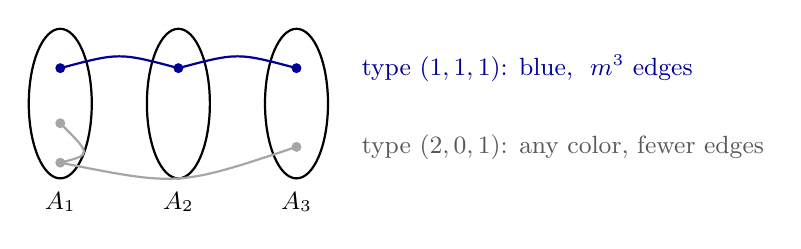
\begin{tikzpicture}[thick, every node/.style={font=\small}]
            \foreach \x/\lab in {0.9/{A_1}, 2.4/{A_2}, 3.9/{A_3}} {
                \draw (\x,1.0) ellipse (0.4 and 0.95);
                \node at (\x,-0.25) {$\lab$};
            }
            \draw[blue!60!black] (0.9,1.45) .. controls (1.65,1.65) .. (2.4,1.45)
                                 (2.4,1.45) .. controls (3.15,1.65) .. (3.9,1.45);
            \foreach \p in {(0.9,1.45),(2.4,1.45),(3.9,1.45)} \fill[blue!60!black] \p circle (1.8pt);
            \node[blue!60!black, anchor=west] at (4.6,1.45) {type $(1,1,1)$: blue, \ $m^3$ edges};
            \draw[gray!70] (0.9,0.75) .. controls (1.3,0.35) .. (0.9,0.25)
                           (0.9,0.25) .. controls (2.4,-0.05) .. (3.9,0.45);
            \foreach \p in {(0.9,0.75),(0.9,0.25),(3.9,0.45)} \fill[gray!70] \p circle (1.8pt);
            \node[gray!70!black, anchor=west] at (4.6,0.45) {type $(2,0,1)$: any color, fewer edges};
        \end{tikzpicture}
    \end{center}

    \textbf{Applying the lemma.} Dividing through by \(m^k\),
    \[
        \mathbb{E}\bigl[ \chi(S) \bigr]
        = m^k \sum_{\substack{(a_1, \ldots, a_k) \\ a_i \ge 0, \ \sum_i a_i = k}}
          \left( \frac{1}{m^k} \sum_{\substack{e \in \binom{A_1 \cup \cdots \cup A_k}{k} \\ e \text{ of type } (a_1, \ldots, a_k)}} \chi(e) \right) p_1^{a_1} \cdots p_k^{a_k}
        = m^k f_\chi(p_1, \ldots, p_k)
    \]
    for a polynomial \(f_\chi\) which is homogeneous of degree \(k\), has all coefficients in \([-1,1]\), and has the coefficient of \(p_1 p_2 \cdots p_k\) equal to \(1\). That is, \(f_\chi \in \mathcal{P}_k\). By \autoref{lem:polynomial} there is a choice of \((p_1, \ldots, p_k) \in [0,1]^k\) with \(\abs{f_\chi(p_1, \ldots, p_k)} \ge c_k\), and we run the random experiment with these probabilities. Then
    \[
        \mathbb{E}\bigl[ \abs{\chi(S)} \bigr] \ge \bigl| \mathbb{E}[\chi(S)] \bigr| \ge c_k m^k,
    \]
    so by \autoref{lem:first-moment} some set \(S \subseteq A_1 \cup \cdots \cup A_k\) satisfies \(\abs{\chi(S)} \ge c_k m^k\). Fix this \(S\).

    \textbf{Reading off the conclusion.} First, \(S\) is large: since \(\abs{\chi(S)}\) is a sum of \(\binom{\abs{S}}{k}\) terms of absolute value \(1\),
    \[
        c_k m^k \le \abs{\chi(S)} \le \binom{\abs{S}}{k} \le \abs{S}^k
        \implies \abs{S} \ge c_k^{1/k} m = \Omega(m) = \Omega\bigl( (\log n)^{1/(k-1)} \bigr).
    \]
    Second, one color dominates on \(S\). Write \(B\) and \(R\) for the numbers of blue and red edges inside \(S\), so \(B + R = \binom{\abs{S}}{k} \eqqcolon N\) and \(\abs{B - R} = \abs{\chi(S)} \ge c_k m^k\). As \(S \subseteq A_1 \cup \cdots \cup A_k\) we have \(\abs{S} \le km\) and hence \(N \le \binom{km}{k} \le \frac{(km)^k}{k!}\). Therefore the majority color occupies a proportion
    \[
        \frac{\max(B,R)}{N} = \frac{1}{2} + \frac{\abs{B-R}}{2N}
        \ \ge\ \frac{1}{2} + \frac{c_k m^k}{2 (km)^k / k!}
        = \frac{1}{2} + \frac{c_k \, k!}{2 k^k}
    \]
    of the edges inside \(S\). The last quantity is a positive constant depending only on \(k\), which is the constant in the statement.
\end{proof}

\chapter{The Method of Alterations}

The first moment principle finds an object that is good \emph{on average}. Often the average object is not quite good enough: a random coloring has a few monochromatic cliques, a random set of vertices spans a few edges, a random set of points contains a few thin triangles. The method of this chapter is to accept those defects and then repair them by hand.

\begin{moral}
    Choose a random structure which is close to having the desired property, and then make a small alteration --- usually deleting one element from each defect --- to establish the property outright.
\end{moral}

The alteration costs something, but if the defects are few the loss is lower order, and we end up with more than the pure first moment gives.
\begin{center}
    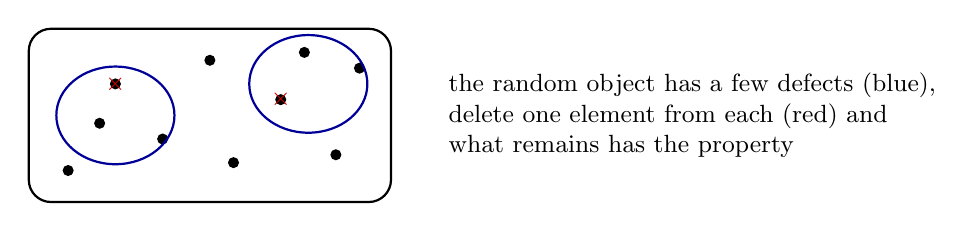
\begin{tikzpicture}[thick, every node/.style={font=\small}]
        \draw[rounded corners=8pt] (0,0) rectangle (4.6,2.2);
        \foreach \x/\y in {0.5/0.4, 1.1/1.5, 1.7/0.8, 2.3/1.8, 2.6/0.5, 3.2/1.3, 3.9/0.6, 4.2/1.7, 0.9/1.0, 3.5/1.9}
            \fill (\x,\y) circle (2pt);
        \draw[blue!60!black] (1.1,1.1) ellipse (0.75 and 0.62);
        \draw[blue!60!black] (3.55,1.5) ellipse (0.75 and 0.62);
        \node[red!80!black] at (1.1,1.5) {$\boldsymbol\times$};
        \node[red!80!black] at (3.2,1.3) {$\boldsymbol\times$};
        \node[anchor=west, align=left] at (5.2,1.1)
            {the random object has a few defects (blue),\\delete one element from each (red) and\\what remains has the property};
    \end{tikzpicture}
\end{center}

\section{Ramsey Numbers Again}\label{sec:ramsey-alteration}

\subsection{What the Union Bound Gives}

We first redo the computation behind \autoref{cor:ramsey-lower} keeping track of the constants, so that there is something to improve on. Recall from \autoref{lem:count-mono} that a uniformly random coloring of \(E(K_n)\) has
\[
    \mathbb{E}[X] = \binom{n}{k} 2^{1 - \binom{k}{2}}
\]
monochromatic copies of \(K_k\) on average, and that \(R(k) > n\) as soon as this is \(< 1\).

\begin{proposition}\label{prop:ramsey-union-sharp}
    \(R(k) \ge (1 - o(1)) \dfrac{k}{e \sqrt{2}} \, 2^{k/2}\).
\end{proposition}

\begin{proof}
    Put \(x \coloneqq \frac{ne}{k \, 2^{(k-1)/2}}\). Using \(\binom{n}{k} \le \bigl( \frac{ne}{k} \bigr)^k\),
    \begin{equation}\label{eq:ramsey-union-x}
        \binom{n}{k} 2^{1 - \binom{k}{2}}
        \le 2 \Bigl( \frac{ne}{k} \Bigr)^{k} 2^{-\frac{k(k-1)}{2}}
        = 2 x^{k}.
    \end{equation}
    By \eqref{eq:ramsey-union-x}, \(\mathbb{E}[X] < 1\) whenever \(2x^k < 1\), i.e.\ \(x < 2^{-1/k}\), i.e.
    \[
        n < y \coloneqq 2^{-1/k} \cdot \frac{k}{e \sqrt{2}} \, 2^{k/2},
    \]
    and by \autoref{cor:ramsey-lower} every such integer \(n\) satisfies \(R(k) > n\). Taking \(n = \lceil y \rceil - 1\) gives \(R(k) \ge \lceil y \rceil \ge y\), that is,
    \[
        R(k) \ge 2^{-1/k} \cdot \frac{k}{e \sqrt{2}} \, 2^{k/2}
        \qquad\text{for every } k.
    \]
    This is the statement: the \(1 - o(1)\) there is exactly the factor \(2^{-1/k} = e^{-(\ln 2)/k} \ge 1 - \frac{\ln 2}{k}\), which tends to \(1\).
\end{proof}

\subsection{Deleting a Vertex from Each Bad Clique}

The union bound throws away everything as soon as \(\mathbb{E}[X] \ge 1\). But a coloring with a handful of monochromatic cliques is nearly as good as one with none: destroy them.

\begin{theorem}\label{thm:ramsey-alteration}
    For every \(k\) and every \(n\),
    \[
        R(k) > n - \binom{n}{k} 2^{1 - \binom{k}{2}}.
    \]
\end{theorem}

\begin{proof}
    Let \(X\) be the number of monochromatic copies of \(K_k\) in a uniformly random red/blue coloring of \(E(K_n)\). Delete one vertex from each monochromatic clique; this removes at most \(X\) vertices, and the coloring induced on the remaining \(\ge n - X\) vertices has no monochromatic \(K_k\) left, since every one of them lost a vertex. Hence
    \[
        R(k) > n - X.
    \]
    By \autoref{lem:count-mono} there is a coloring with \(X \le \mathbb{E}[X] = \binom{n}{k} 2^{1-\binom{k}{2}}\), and using that coloring gives the bound.
\end{proof}

Now we are free to choose \(n\) as large as we like, and the right choice is the one maximising the right-hand side rather than the one making it positive.

\begin{corollary}\label{cor:ramsey-alteration}
    \(R(k) \ge (1 - o(1)) \dfrac{k}{e} \, 2^{k/2}\).
\end{corollary}

\begin{proof}
    Write \(c = \bigl( \frac{e}{k} \bigr)^{k} 2^{1 - \binom{k}{2}}\), so that \autoref{thm:ramsey-alteration} together with \(\binom{n}{k} \le \bigl( \frac{ne}{k} \bigr)^k\) gives \(R(k) > n - c n^k\). Differentiating with respect to \(n\),
    \[
        1 - k c \, n^{k-1} = 0
        \iff n^{k-1} = \frac{1}{kc} = \frac{k^{k-1}}{e^{k}} \, 2^{\binom{k}{2} - 1}
        \iff n = (1-o(1)) \frac{k}{e} \, 2^{k/2},
    \]
    where for the last step we take \((k-1)\)-th roots factor by factor, using \(\binom{k}{2}/(k-1) = \frac{k}{2}\):
    \[
        n
        = \underbrace{\bigl(k^{k-1}\bigr)^{\frac{1}{k-1}}}_{=\,k}
        \cdot \underbrace{\bigl(e^{-k}\bigr)^{\frac{1}{k-1}}}_{=\,e^{-1} \, e^{-\frac{1}{k-1}}}
        \cdot \underbrace{\bigl(2^{\binom{k}{2} - 1}\bigr)^{\frac{1}{k-1}}}_{=\,2^{k/2} \, 2^{-\frac{1}{k-1}}}
        = \underbrace{(2e)^{-\frac{1}{k-1}}}_{\to\, 1} \cdot \frac{k}{e} \, 2^{k/2}.
    \]
    At this \(n\) we have \(c n^{k} = \frac{n}{k}\), so
    \[
        R(k) > n - \frac{n}{k} = \Bigl( 1 - \frac{1}{k} \Bigr) n = (1-o(1)) \frac{k}{e} \, 2^{k/2}. \qedhere
    \]
\end{proof}

\begin{remark}
    The alteration gained exactly a factor \(\sqrt{2}\) over \autoref{prop:ramsey-union-sharp}, and nothing more: the exponential rate \(2^{k/2}\) is untouched. This is typical. Determining whether the rate itself can be improved is a famous open problem; the best known bounds are still of the form \(2^{(\frac{1}{2} + o(1))k} \le R(k) \le 2^{(2 - o(1))k}\) in the exponent.
\end{remark}

\section{Independent Sets and Tur\'an's Theorem}\label{sec:turan}

\begin{recall}
    \autoref{thm:mantel}: an \(n\)-vertex graph with more than \(\frac{n^2}{4}\) edges contains a triangle.
\end{recall}

Tur\'an's theorem is the generalisation of \autoref{thm:mantel} from triangles to \(K_k\).

\begin{theorem}[Tur\'an, 1941]\label{thm:turan}
    If \(G\) is an \(n\)-vertex graph with more than \(\bigl( 1 - \frac{1}{k-1} \bigr) \frac{n^2}{2}\) edges, then \(G\) contains \(K_k\).
\end{theorem}

\begin{definition}[Independence number]\label{def:independence}
    The \vocab{independence number} \(\alpha(G)\) is the largest number of vertices of \(G\) spanning no edge.
\end{definition}

Passing to the complement \(\overline{G}\) turns cliques into independent sets, and \(G\) has more than \(\bigl( 1 - \frac{1}{k-1} \bigr) \frac{n^2}{2}\) edges iff \(\overline{G}\) has fewer than
\[
    \binom{n}{2} - \Bigl( 1 - \frac{1}{k-1} \Bigr) \frac{n^2}{2} = \frac{n^2}{2(k-1)} - \frac{n}{2}
\]
edges, which is \(\frac{1}{k-1} \binom{n}{2}\) up to lower-order terms. So \autoref{thm:turan} has an equivalent form, which is the one we shall prove.

\begin{theorem}[Tur\'an, 1941; complementary form]\label{thm:turan-complement}
    If \(G\) is an \(n\)-vertex graph with \(\lesssim \frac{1}{k-1} \binom{n}{2}\) edges, then \(\alpha(G) \ge k\).
\end{theorem}

Throughout this section \(G\) has \(n\) vertices and \(m\) edges, and the benchmark to keep in mind is
\[
    m \approx \frac{1}{k-1} \binom{n}{2} \approx \frac{n^2}{2(k-1)},
\]
for which we are trying to produce an independent set of size about \(k\). We give three attempts, each stronger than the last.

\subsection{Attempt 1: A Random Subset}

Let \(S \subseteq V(G)\) be a random subset, each vertex included independently with probability \(p\), and let \(X\) be the number of edges inside \(S\). Then
\[
    X = \sum_{e \in E(G)} X_e, \qquad
    X_e = \begin{cases} 1, & \text{if } e \subseteq S, \\ 0, & \text{if } e \not\subseteq S, \end{cases}
    \qquad \mathbb{P}(e \subseteq S) = p^2,
\]
so by \autoref{thm:linearity}
\[
    \mathbb{E}[X] = \sum_{e \in E(G)} \mathbb{E}[X_e] = \sum_{e \in E(G)} \mathbb{P}(e \subseteq S) = m p^2.
\]
If \(mp^2 < 1\), i.e.\ \(p < \frac{1}{\sqrt{m}}\), then by \autoref{lem:first-moment} some outcome has \(X \le \mathbb{E}[X] < 1\), hence \(X = 0\), i.e.\ \(S\) is independent. By itself this says nothing about \(\abs{S}\): \(S = \varnothing\) is also independent. The heuristic is to \emph{pretend} that this independent \(S\) has the typical size of \(\abs{S} \sim \operatorname{Bin}(n,p)\), namely \(\mathbb{E}\abs{S} = np\). Taking \(p\) just below \(\frac{1}{\sqrt{m}}\) would then give
\[
    \alpha(G) \ge \abs{S} \approx np \approx \frac{n}{\sqrt{m}},
\]
and at the benchmark \(m \approx \frac{n^2}{2(k-1)}\), i.e.\ \(\sqrt{m} \approx \frac{n}{\sqrt{2(k-1)}}\),
\[
    \frac{n}{\sqrt{m}} \approx \sqrt{2(k-1)}.
\]
Two things are wrong with this. The conclusion is only of order \(\sqrt{k}\) instead of \(k\); and the argument is not even complete, since the pretending step is unjustified: we would need one outcome with both \(X = 0\) and \(\abs{S} \approx np\), i.e.\ \(\mathbb{P}\bigl( X = 0, \ \abs{S} \ge (1-\varepsilon) np \bigr) > 0\), which needs a concentration bound on \(\abs{S}\). The next attempt repairs both at once.

\subsection{Attempt 2: Alterations}

We do not need \(S\) to be independent --- it is enough that \(S\) has \emph{few} edges, because we can then delete one endpoint from each edge and what remains is independent.

\begin{center}
    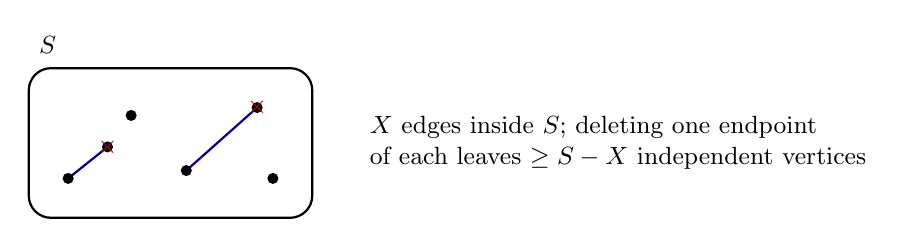
\begin{tikzpicture}[thick, every node/.style={font=\small}]
        \draw[rounded corners=8pt] (0,0) rectangle (3.6,1.9);
        \node[anchor=south west] at (0,1.95) {$S$};
        \coordinate (p1) at (0.5,0.5); \coordinate (p2) at (1.3,1.3);
        \coordinate (p3) at (2.0,0.6);  \coordinate (p4) at (2.9,1.4);
        \coordinate (p5) at (1.0,0.9);  \coordinate (p6) at (3.1,0.5);
        \draw[blue!60!black] (p1) -- (p5) (p3) -- (p4);
        \foreach \p in {p1,p2,p3,p4,p5,p6} \fill (\p) circle (2pt);
        \node[red!80!black] at (1.0,0.9) {$\boldsymbol\times$};
        \node[red!80!black] at (2.9,1.4) {$\boldsymbol\times$};
        \node[anchor=west, align=left] at (4.2,0.95)
            {\(X\) edges inside \(S\); deleting one endpoint\\of each leaves \(\ge \abs{S} - X\) independent vertices};
    \end{tikzpicture}
\end{center}

So for \emph{every} set \(S\), writing \(X = X(S)\) for the number of edges inside it,
\[
    \alpha(G) \ge \abs{S} - X(S),
\]
and we may take expectations instead of hoping for a single good outcome:
\[
    \alpha(G) \ge \mathbb{E}\bigl[ \abs{S} - X \bigr] = \mathbb{E}\bigl[ \abs{S} \bigr] - \mathbb{E}[X] = np - mp^2,
\]
using \autoref{lem:first-moment} and \autoref{thm:linearity}. Now choose \(p\) to maximise: differentiating, \(n - 2pm = 0\), i.e.\ \(p = \frac{n}{2m}\), which lies in \([0,1]\) provided \(m \ge \frac{n}{2}\). Plugging in,
\[
    \alpha(G) \ge \frac{n^2}{2m} - m \cdot \frac{n^2}{4m^2} = \frac{n^2}{4m}.
\]
At the benchmark \(m \approx \frac{n^2}{2(k-1)}\) this gives
\[
    \alpha(G) \ge \frac{k-1}{2},
\]
of the right order in \(k\), but still a factor \(2\) away from \autoref{thm:turan-complement}.

\subsection{Attempt 3: A Random Greedy Algorithm}

The last factor \(2\) is recovered by not throwing vertices away at all, but by building the independent set greedily in a random order.

\begin{notation}
    \(\deg(v)\) is the degree of \(v\) in \(G\), and \(N(v)\) its neighbourhood.
\end{notation}

The algorithm is:
\begin{enumerate}[(1)]
    \item order the vertices \(v_1, v_2, \ldots, v_n\) uniformly at random;
    \item going along the order, add \(v_i\) to the independent set \(I\) if it is not adjacent to any previously chosen vertex.
\end{enumerate}
By construction \(I\) is independent. Let \(X = \abs{I}\), and decompose it over the vertices:
\[
    X = \sum_{v \in V(G)} X_v, \qquad
    X_v = \begin{cases} 1, & \text{if } v \in I, \\ 0, & \text{if } v \notin I, \end{cases}
    \qquad \text{so} \qquad
    \mathbb{E}[X] = \sum_{v \in V(G)} \mathbb{P}(v \in I).
\]

\begin{observation}\label{obs:caro-wei-prob}
    \(\mathbb{P}(v \in I) \ge \mathbb{P}(v \text{ comes before all of its neighbours}) = \dfrac{1}{1 + \deg(v)}\).
\end{observation}

Indeed, if \(v\) precedes all of \(N(v)\) then none of its neighbours has been chosen when \(v\) is examined, so \(v\) joins \(I\); and among the \(1 + \deg(v)\) vertices of \(\{v\} \cup N(v)\), each is equally likely to come first in a uniformly random order. The inequality is not an equality, since \(v\) can also be chosen when a neighbour precedes it but was itself rejected.
\begin{center}
    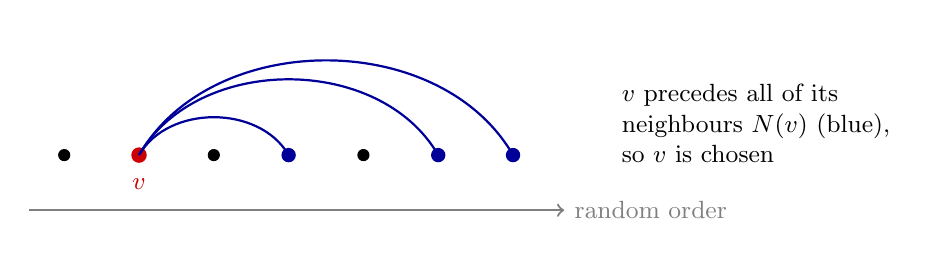
\begin{tikzpicture}[thick, every node/.style={font=\small}]
        \foreach \i in {1,...,7} \coordinate (o\i) at (0.95*\i,0);
        \foreach \i in {1,...,7} \fill (o\i) circle (2.2pt);
        \draw[->, gray] (0.5,-0.7) -- (7.3,-0.7) node[right, gray] {random order};
        \fill[red!80!black] (o2) circle (2.8pt);
        \node[red!80!black, below=5pt] at (o2) {$v$};
        \foreach \i in {4,6,7} {
            \fill[blue!60!black] (o\i) circle (2.6pt);
            \draw[blue!60!black] (o2) to[out=60, in=120] (o\i);
        }
        \node[anchor=west, align=left] at (7.9,0.4)
            {\(v\) precedes all of its\\neighbours \(N(v)\) (blue),\\so \(v\) is chosen};
    \end{tikzpicture}
\end{center}

\begin{theorem}[Caro--Wei]\label{thm:caro-wei}
    For any graph \(G\),
    \[
        \alpha(G) \ge \sum_{v \in V(G)} \frac{1}{1 + \deg(v)}.
    \]
\end{theorem}

\begin{proof}
    By \hyperref[obs:caro-wei-prob]{the Observation above} and \autoref{thm:linearity}, \(\mathbb{E}[X] \ge \sum_{v} \frac{1}{1+\deg(v)}\), and by \autoref{lem:first-moment} some order produces an independent set at least this large.
\end{proof}

\begin{corollary}\label{cor:caro-wei}
    If \(G\) is an \(n\)-vertex graph with \(m\) edges, then
    \[
        \alpha(G) \ge \frac{n}{1 + \frac{2m}{n}}.
    \]
\end{corollary}

\begin{proof}
    Recall Jensen's inequality: if \(\varphi\) is convex on an interval \(I\) and \(x_1, \ldots, x_n \in I\), then
    \[
        \frac{1}{n} \sum_{i=1}^{n} \varphi(x_i) \ge \varphi\Bigl( \frac{1}{n} \sum_{i=1}^{n} x_i \Bigr).
    \]
    Apply it with \(\varphi(x) = \frac{1}{1+x}\), which is convex on \([0,\infty)\) since \(\varphi''(x) = \frac{2}{(1+x)^3} > 0\), and with the \(x_i\) the degrees \(\deg(v)\). By the handshake lemma \(\sum_{v} \deg(v) = 2m\), so the average degree is \(\frac{2m}{n}\) and
    \[
        \sum_{v \in V(G)} \frac{1}{1 + \deg(v)} \ge n \, \varphi\Bigl( \frac{2m}{n} \Bigr) = \frac{n}{1 + \frac{2m}{n}},
    \]
    which together with \autoref{thm:caro-wei} gives the claim.
\end{proof}

At the benchmark \(m = \frac{1}{k-1} \binom{n}{2}\) we have \(\frac{2m}{n} = \frac{n-1}{k-1}\), and
\[
    \alpha(G) \ge \frac{n}{1 + \frac{n-1}{k-1}} = \frac{n(k-1)}{n + k - 2} = (1 - o(1)) (k-1),
\]
which is \autoref{thm:turan-complement}.

\begin{remark}
    \autoref{cor:caro-wei} is sharp. Let \((k-1) \mid n\) and let \(G\) be the disjoint union of \(k-1\) copies of \(K_{n/(k-1)}\). Every vertex has degree \(\frac{n}{k-1} - 1\), so \(\frac{2m}{n} = \frac{n}{k-1} - 1\) and the bound of \autoref{cor:caro-wei} reads
    \[
        \alpha(G) \ge \frac{n}{1 + \frac{2m}{n}} = \frac{n}{n/(k-1)} = k - 1.
    \]
    On the other hand \(\alpha(G) \le k-1\): two vertices in the same clique are adjacent, so an independent set has at most one vertex from each of the \(k-1\) cliques. Hence \(\alpha(G) = k-1\) and the bound is attained.

    The complement \(\overline{G}\) is the complete \((k-1)\)-partite graph with equal parts, which is \(K_k\)-free (a clique in \(\overline{G}\) is an independent set in \(G\)) and has exactly \(\bigl(1 - \frac{1}{k-1}\bigr) \frac{n^2}{2}\) edges; it is the extremal graph of \autoref{thm:turan}.

    Comparing the three attempts at the benchmark:
    \[
        \underbrace{\sqrt{2(k-1)}}_{\text{Attempt 1}}
        \ <\ \underbrace{\frac{k-1}{2}}_{\text{Attempt 2}}
        \ <\ \underbrace{k-1}_{\text{Attempt 3}} \quad (\text{for large } k),
    \]
    and by the example above the last cannot be improved.
\end{remark}

\section{The Heilbronn Triangle Problem}\label{sec:heilbronn}

\begin{question}\label{q:heilbronn}
    If we place \(n\) points in \([0,1]^2\), how small must the smallest triangle they span be?
\end{question}

Three points taken at random usually span a triangle of constant area, but with many points some triple is bound to be nearly collinear. The question is how nearly, and the alteration method gives a good lower bound with no construction at all.

\begin{proposition}\label{prop:heilbronn}
    There is a set of \(n\) points in \([0,1]^2\) s.t.\ every triangle spanned by three of them has area \(\ge \frac{1}{100 n^2}\).
\end{proposition}

The proof needs one geometric estimate, which is where the areas enter.

\begin{lemma}\label{lem:thin-triangle}
    Let \(A, B, C\) be three independent uniformly random points of \([0,1]^2\), and let \(E\) be the event that the triangle \(ABC\) has area \(\le \varepsilon\). Then \(\mathbb{P}(E) \le 16 \pi \varepsilon\).
\end{lemma}

\begin{proof}
    Condition on \(A\) and \(B\) with \(\abs{AB} = b\). The area of \(ABC\) is \(\frac{1}{2} b \cdot \dist(C, AB)\), so \(E\) occurs iff \(C\) lies in the strip of half-width \(\frac{2\varepsilon}{b}\) around the line \(AB\). That strip meets \([0,1]^2\) in a set of length at most \(\sqrt{2}\), the diameter of the square, so
    \[
        \mathbb{P}\bigl( E \mid \abs{AB} = b \bigr) \le \sqrt{2} \cdot \frac{4 \varepsilon}{b}.
    \]
    \begin{center}
        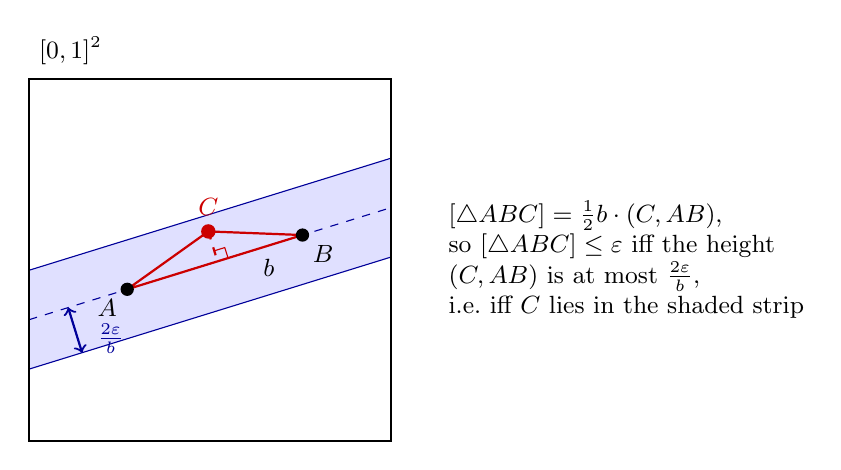
\begin{tikzpicture}[thick, every node/.style={font=\small}]
            % the strip, clipped to the unit square
            \begin{scope}
                \clip (0,0) rectangle (4.6,4.6);
                \fill[blue!12] (-0.577,1.987) -- (4.823,3.659) -- (5.177,2.513) -- (-0.223,0.841) -- cycle;
                \draw[blue!60!black, thin] (-0.577,1.987) -- (4.823,3.659);
                \draw[blue!60!black, thin] (-0.223,0.841) -- (5.177,2.513);
                \draw[blue!60!black, thin, dashed] (-0.4,1.414) -- (5.0,3.086);
            \end{scope}
            \draw (0,0) rectangle (4.6,4.6);
            \node[anchor=south west] at (0,4.65) {$[0,1]^2$};
            % the triangle
            \coordinate (A) at (1.25,1.925);
            \coordinate (B) at (3.476,2.614);
            \coordinate (C) at (2.28,2.66);
            \coordinate (F) at (2.397,2.280);
            \draw[red!80!black] (A) -- (B) -- (C) -- cycle;
            \draw[red!80!black, dashed] (C) -- (F);
            \draw[red!80!black, thin] (2.531,2.321) -- (2.489,2.455) -- (2.356,2.414);
            \fill (A) circle (2.4pt) node[below left=0pt] {$A$};
            \fill (B) circle (2.4pt) node[below right=0pt] {$B$};
            \fill[red!80!black] (C) circle (2.6pt);
            \node[red!80!black, above=2pt] at (C) {$C$};
            \node[anchor=north] at (3.05,2.44) {$b$};
            % the half-width of the strip, measured perpendicular to AB
            \draw[<->, blue!60!black] (0.5,1.693) -- (0.677,1.120);
            \node[blue!60!black, anchor=west] at (0.74,1.30) {$\frac{2\varepsilon}{b}$};
            \node[anchor=west, align=left] at (5.2,2.3)
                {\([\triangle ABC] = \frac{1}{2} b \cdot \dist(C, AB)\),\\so \([\triangle ABC] \le \varepsilon\) iff the height\\\(\dist(C, AB)\) is at most \(\frac{2\varepsilon}{b}\),\\i.e.\ iff \(C\) lies in the shaded strip};
        \end{tikzpicture}
    \end{center}
    Next we bound the density \(f_{\abs{AB}}\) of \(\abs{AB}\). Fix \(A\). Then \(b < \abs{AB} \le b+h\) iff \(B\) lies in the annulus centred at \(A\) with radii \(b\) and \(b+h\). Since \(B\) is uniform on \([0,1]^2\), which has area \(1\), the probability that \(B\) lands in a region is the area of that region inside the square, which is at most the area of the whole annulus. This holds for every \(A\), hence also after averaging over \(A\):
    \[
        \mathbb{P}\bigl( b < \abs{AB} \le b+h \bigr) \le \pi (b+h)^2 - \pi b^2 = 2\pi b h + \pi h^2.
    \]
    \begin{center}
        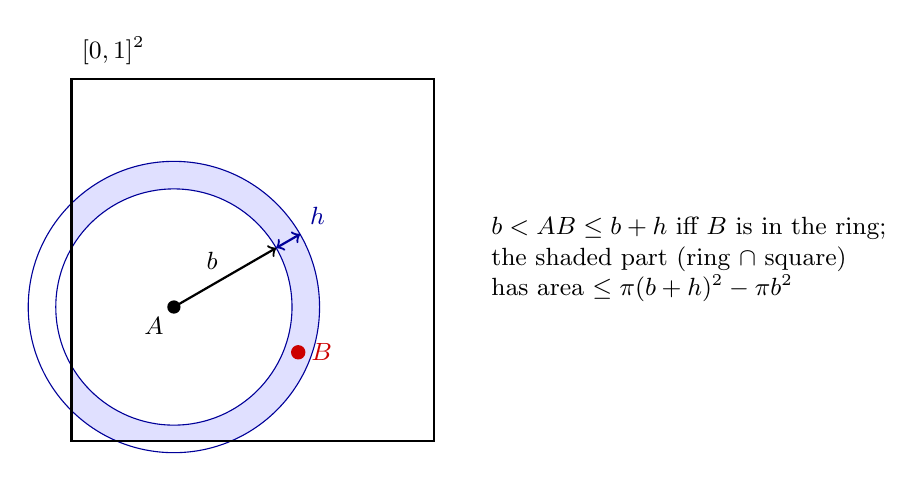
\begin{tikzpicture}[thick, every node/.style={font=\small}]
            \coordinate (A) at (1.3,1.7);
            \begin{scope}
                \clip (0,0) rectangle (4.6,4.6);
                \fill[blue!12, even odd rule] (A) circle (1.85) (A) circle (1.5);
            \end{scope}
            \draw[blue!60!black, thin] (A) circle (1.5);
            \draw[blue!60!black, thin] (A) circle (1.85);
            \draw (0,0) rectangle (4.6,4.6);
            \node[anchor=south west] at (0,4.65) {$[0,1]^2$};
            \draw[->] (A) -- (2.599,2.45) node[midway, above left=-1pt] {$b$};
            \draw[<->, blue!60!black] (2.599,2.45) -- (2.902,2.625);
            \node[blue!60!black, anchor=south west] at (2.9,2.62) {$h$};
            \fill (A) circle (2.4pt) node[below left=0pt] {$A$};
            \fill[red!80!black] (2.879,1.125) circle (2.6pt) node[right=1pt] {$B$};
            \node[anchor=west, align=left] at (5.2,2.3)
                {\(b < \abs{AB} \le b+h\) iff \(B\) is in the ring;\\the shaded part (ring \(\cap\) square)\\has area \(\le \pi(b+h)^2 - \pi b^2\)};
        \end{tikzpicture}
    \end{center}
    Dividing by \(h\) and letting \(h \to 0\),
    \[
        f_{\abs{AB}}(b) = \lim_{h \to 0} \frac{\mathbb{P}\bigl( b < \abs{AB} \le b+h \bigr)}{h} \le \lim_{h \to 0} \, (2\pi b + \pi h) = 2\pi b.
    \]
    Since \(\abs{AB} \le \sqrt{2}\) always,
    \[
        \mathbb{P}(E) = \int_{0}^{\sqrt{2}} f_{\abs{AB}}(b) \, \mathbb{P}\bigl( E \mid \abs{AB} = b \bigr) \, \dd b
        \le \int_{0}^{\sqrt{2}} 2\pi b \cdot \frac{4\sqrt{2}\, \varepsilon}{b} \, \dd b
        = 8\sqrt{2} \pi \varepsilon \cdot \sqrt{2} = 16 \pi \varepsilon. \qedhere
    \]
\end{proof}

\begin{proof}[Proof of \autoref{prop:heilbronn}]
    Let \(P_1, \ldots, P_{2n}\) be independent uniformly random points of \([0,1]^2\) --- note that we start with twice as many points as we want --- and let \(X\) be the number of triangles of area at most \(\varepsilon\) among them:
    \[
        X = \sum_{1 \le i < j < l \le 2n} X_{ijl}, \qquad
        X_{ijl} = \begin{cases} 1, & \text{if } [\triangle P_i P_j P_l] \le \varepsilon, \\ 0, & \text{otherwise}. \end{cases}
    \]
    By \autoref{thm:linearity} and \autoref{lem:thin-triangle},
    \[
        \mathbb{E}[X] = \sum_{1 \le i < j < l \le 2n} \mathbb{E}[X_{ijl}] = \binom{2n}{3} \, \mathbb{P}\bigl( [\triangle P_1 P_2 P_3] \le \varepsilon \bigr) \le \binom{2n}{3} 16 \pi \varepsilon.
    \]
    Choose \(\varepsilon = \frac{1}{100 n^2}\). Then, as \(\binom{2n}{3} \le \frac{4n^3}{3}\),
    \[
        \mathbb{E}[X] \le \frac{4 n^3}{3} \cdot \frac{16 \pi}{100 n^2} = \frac{64 \pi}{300} \, n \le n,
    \]
    so by \autoref{lem:first-moment} there are \(2n\) points spanning at most \(n\) triangles of area \(\le \varepsilon\). Now alter: delete one point from each such triangle. At least \(2n - n = n\) points remain, and no three of them span a triangle of area \(\le \varepsilon = \frac{1}{100n^2}\).
\end{proof}

\begin{remark}\hfill
    \begin{enumerate}[(1)]
        \item Erd\H{o}s gave a deterministic construction whose smallest triangle has area \(\Omega\bigl( \frac{1}{n^2} \bigr)\); see the homework.
        \item Heilbronn conjectured that \(\Theta\bigl( \frac{1}{n^2} \bigr)\) is best possible.
        \item This is false: Koml\'os, Pintz and Szemer\'edi (1982) produced \(n\) points in \([0,1]^2\) in which every triangle has area \(\Omega\bigl( \frac{\log n}{n^2} \bigr)\), by a probabilistic argument.
    \end{enumerate}
\end{remark}

\section{Large Chromatic Number}\label{sec:chromatic}

\begin{definition}[Chromatic number]\label{def:chromatic}
    Given a graph \(G\), the \vocab{chromatic number} \(\chi(G)\) is the least number of colors needed to color the vertices so that no edge is monochromatic, i.e.\ so that adjacent vertices receive different colors.
\end{definition}

Equivalently, \(\chi(G)\) is the least number of independent sets into which \(V(G)\) can be partitioned, the color classes.
\begin{center}
    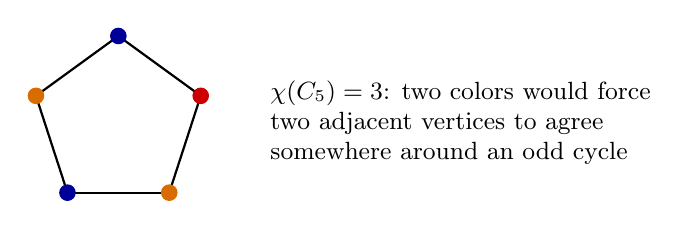
\begin{tikzpicture}[thick, every node/.style={font=\small}]
        \foreach \i in {1,...,5} \coordinate (c\i) at ({90+72*(\i-1)}:1.1);
        \foreach \i [evaluate=\i as \j using {int(mod(\i,5)+1)}] in {1,...,5}
            \draw (c\i) -- (c\j);
        \foreach \i/\col in {1/{blue!60!black}, 2/{orange!85!black}, 3/{blue!60!black}, 4/{orange!85!black}, 5/{red!80!black}}
            \fill[\col] (c\i) circle (3pt);
        \node[anchor=west, align=left] at (1.8,0)
            {\(\chi(C_5) = 3\): two colors would force\\two adjacent vertices to agree\\somewhere around an odd cycle};
    \end{tikzpicture}
\end{center}

Two bounds are immediate.

\begin{proposition}\label{prop:chromatic-bounds}
    For every graph \(G\),
    \begin{enumerate}[(1)]
        \item \(\chi(G) \ge \omega(G) \coloneqq \max\{ k : K_k \subseteq G \}\), the \vocab{clique number};
        \item \(\chi(G) \ge \dfrac{\abs{V(G)}}{\alpha(G)}\).
    \end{enumerate}
\end{proposition}

\begin{proof}
    (1) The vertices of a clique are pairwise adjacent, so they must all receive different colors.

    (2) Every color class is an independent set, hence of size at most \(\alpha(G)\), and the classes cover all \(\abs{V(G)}\) vertices.
\end{proof}
